\documentclass[alternative-exam.tex]{subfiles}
\begin{document}

\chapter{Matchmaker}
Een matchmaking bureau wil een systeem maken dat hen zegt of een potenti\"ele partner al dan niet goed is voor een bepaalde cli\"ent. Ze ontwikkelen uiteindelijk een systeem dat machine learning gebruikt om te voorspellen hoe de cli\"ent een potentiele partner zal beoordelen.

\section{Vraag}
Het bureau vraagt kandidaten een aantal persoonlijke eigenschappen op te geven.
De specifieke mogelijkheden zijn voor elke eigenschap beperkt.
\begin{itemize}
\item Geslacht: man / vrouw
\item Leeftijd: jonger / zelfde / ouder\footnote{De kandidaat moet zijn leeftijd opgeven, maar het systeem houdt enkel bij of de kandidaat jonger of ouder is dan de cli\"ent, of ongeveer dezelfde leeftijd heeft als de cli\"ent.}
\item Muziek: pop / latin / jazz  / klassiek
\item Sport: tennis / golf / joggen / fitness / voetbal
\end{itemize}
De cli\"ent heeft de vorige kandidaten beoordeeld zoals beschreven in figuur \ref{beoordeling}
\begin{figure}[H]
\centering
\caption{Beoordeling}
\label{beoordeling}
\begin{tabular}{|c|c|c|c|c|}
\hline
geslacht & leeftijd & muziek & sport & beoordeling\\
\hline
vrouw & zelfde & jazz & voetbal & +\\
man & jonger & pop & joggen & -\\%
vrouw & ouder & pop & fitness & -\\
vrouw & jonger & klassiek & golf & +\\
vrouw & zelfde & latin & tennis & +\\
\hline
\end{tabular}
\end{figure}
Aan de hand van de formulering van het systeem heeft het IT departement een hypothesetaal opgesteld zoals beschreven in figuur \ref{hypothesetaal}.
\begin{figure}[H]
\centering
\caption{Hypothesetaal}
\label{hypothesetaal}
\begin{tikzpicture}
\node (s) at (-4,-0.5) {\small Geslacht};
\node (sG) at (-4,-1) {\small ?};
\node (si) at (-5,-2.5) {\small man \tiny m};
\draw[->] (sG) -- (si);
\node (sw) at (-3,-2.5) {\small vrouw \tiny v};
\draw[->] (sG) -- (sw);

\node (a) at (4,-0.5) {\small Leeftijd};
\node (aG) at (4,-1) {\small ?};
\node (ay) at (2.5,-2.5) {\small jonger \tiny j};
\draw[->] (aG) -- (ay);
\node (am) at (4,-2.5) {\small zelfde \tiny z};
\draw[->] (aG) -- (am);
\node (ao) at (5.5,-2.5) {\small ouder\tiny o};
\draw[->] (aG) -- (ao);
\end{tikzpicture}\\\vspace{1cm}
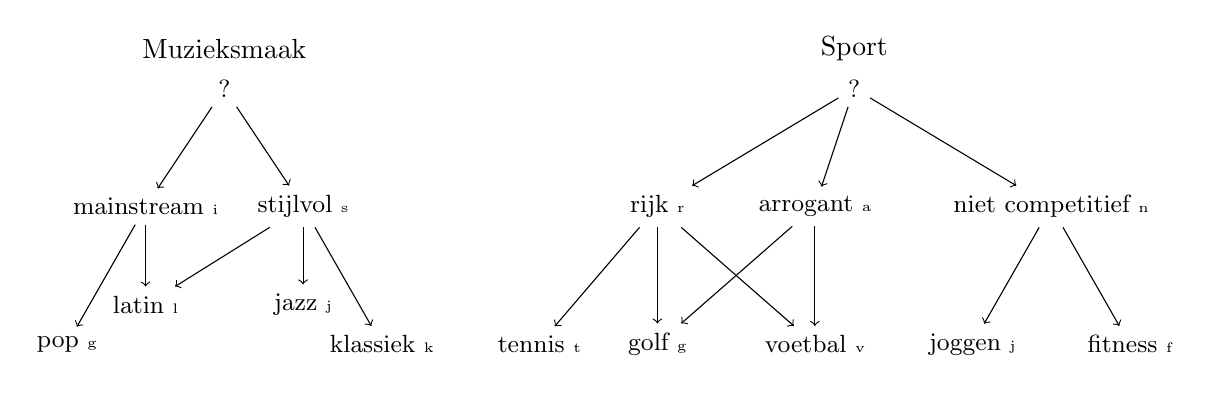
\begin{tikzpicture}
\node (h) at (-4,-0.5) {Muzieksmaak};
\node (hG) at (-4,-1) {\small ?};
\node (hi) at (-5,-2.5) {\small mainstream \tiny i};
\draw[->] (hG) -- (hi);
\node (hig) at (-6,-4.25) {\small pop \tiny g};
\draw[->] (hi) -- (hig);
\node (hil) at (-5,-3.75) {\small latin \tiny l};
\draw[->] (hi) -- (hil);
\node (hr) at (-3,-2.5) {\small stijlvol \tiny s};
\draw[->] (hG) -- (hr);
\draw[->] (hr) -- (hil);
\node (hrs) at (-3,-3.75) {\small jazz \tiny j};
\draw[->] (hr) -- (hrs);
\node (hrf) at (-2,-4.25) {\small klassiek \tiny k};
\draw[->] (hr) -- (hrf);
%\draw (0,0.5) -- (0,-5);
\node (h) at (4,-0.5) {Sport};
\node (hG) at (4,-1) {\small ?};

\node (hi) at (1.5,-2.5) {\small rijk \tiny r};
\draw[->] (hG) -- (hi);
\node (hig) at (0,-4.25) {\small tennis \tiny t};
\draw[->] (hi) -- (hig);
\node (hil) at (1.5,-4.25) {\small golf \tiny g};
\draw[->] (hi) -- (hil);
\node (hv) at (3.5,-2.5) {\small arrogant \tiny a};
\draw[->] (hG) -- (hv);
\node (hiv) at (3.5,-4.25) {\small voetbal \tiny v};
\draw[->] (hv) -- (hiv);
\draw[->] (hi) -- (hiv);
\draw[->] (hv) -- (hil);
\node (hr) at (6.5,-2.5) {\small niet competitief \tiny n};
\draw[->] (hG) -- (hr);
\node (hrs) at (5.5,-4.25) {\small joggen \tiny j};
\draw[->] (hr) -- (hrs);
\node (hrf) at (7.5,-4.25) {\small fitness \tiny f};
\draw[->] (hr) -- (hrf);

\end{tikzpicture}
\end{figure}
Aan het eind van de dag komt er een dame binnen die jonger is dan de cli\"ent, naar jazzmuziek luistert, en elke week gaat joggen. Is deze dame een goede match voor de cli\"ent, volgens het systeem?

\section{Modeloplossing}
% TODO toevoegen wat S is, wat G is, wat de vormen van de nodes betekenen.
We voeren het version-spaces algoritme uit op de voorbeelden uit de opgave (zie \ref{versionspaces}). We beginnen met het initialiseren van $S$ en $G$. $S$ bevat initieel enkel de hypothese die met alles inconsistent is. $G$ daarentegen, bevat de hypothese die met alles consistent is.
\[
S = \{\bot\}
\]
\[
G = \{[?,?,?,?]\}
\]
De hypothesen die in $S$ en $G$ zitten zijn na elke iteratie getekend in een graaf. De graag bestaat uit twee bomen waarvan de bovenste $S$ voorstelt en de onderste $G$. Niet alle hypothesen die getekend zijn zitten echter in $G$ of in $S$. Als een hypothese niet in \'e\'en van de verzamelingen zit wordt het met een ellips afgebeeld. De rechthoekige nodes zitten wel in $G$ of $S$.
\subsection{Iteratie 1}
\begin{figure}
[H]
\centering
\caption{Iteratie 1}
\label{iter_1}
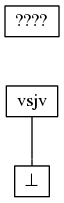
\includegraphics[scale=0.5]{resources/graphs/iteration_1.png}
\end{figure}
Het eerste voorbeeld is een positief voorbeeld. We generaliseren alle hypothesen in $S$ waaraan het voorbeeld niet voldoet. $\bot$ wordt dus gegeneraliseerd naar de hypothese die het voorbeeld precies omvat. Het resultaat zien we in figuur \ref{iter_1}.
\begin{itemize}
\item $G = \{[?,?,?,?]\}$
\item $S = \{[v,z,j,v]\}$
\end{itemize}

\subsection{Iteratie 2}
\begin{figure}
[H]
\centering
\caption{Iteratie 2}
\label{iter_2}
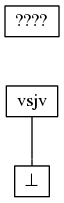
\includegraphics[scale=0.5]{resources/graphs/iteration_2.png}
\end{figure}
Het volgende voorbeeld is negatief beoordeeld. We specifi\"eren alle hypothesen in $G$ waaraan het voorbeeld voldoet. $[m,j,p,g]$ voldoet aan $[?,?,?,?]$ dus we moeten dit specifi\"eren tot het voorbeeld net niet meer aan die nieuwe hypothese(n) voldoet. We voegen in totaal zes hypothesen toe onder $[?,?,?,?]$. Nu begint het snoeien. We verwijderen $[?,o,?,?]$ en $[?,?,?,f]$ omdat deze hypothesen inconsistent zijn met $[v,z,j,v]$. Een overzicht van deze iteratie zien we in figuur \ref{iter_2}.
\begin{itemize}
\item $G = \{[v,?,?,?],[?,z,?,?],[?,?,s,?],[?,?,?,r]\}$
\item $S = \{[v,z,j,v]\}$
\item Gesnoeid: $[?,o,?,?],[?,?,?,f]$
\end{itemize}

\subsection{Iteratie 3}
\begin{sidewaysfigure}
\centering
\caption{Iteratie 3}
\label{iter_3}
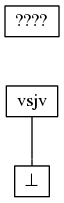
\includegraphics[scale=0.35]{resources/graphs/iteration_3.png}
\end{sidewaysfigure}
Voorbeeld $3$ is opnieuw negatief beoordeeld. We voeren opnieuw de bovenstaande procedure uit. Deze keer worden er weer een aantal hypothesen gesnoeid, maar we kunnen nu ook enkele hypothesen verwijderen omdat ze redundant zijn. $[?,z,j,?]$ en $[?,z,?,v]$ zijn respectievelijk specificaties van $[?,?,s,?]$ en $[?,?,?,r]$ en kunnen daarom ook verwijderd worden uit $G$. Zie figuur \ref{iter_3} voor het volledige overzicht van deze iteratie.
\begin{itemize}
\item $G = \{[?,v,?,j],[v,?,?,r],[?,z,j,?],[?,z,?,v]\}$
\item $S = \{[v,z,j,v]\}$
\item Gesnoeid: $[v,j,?,?]$, $[v,o,?,?]$, $[v,?,m,?]$, $[v,?,?,j]$, $[m,z,?,?]$, $[?,z,m,?]$, $[?,z,?,t]$,

$[?,z,?,n]$ en $[?,z,j,?]$, $[?,z,?,v]$
\end{itemize}
\subsection{Iteratie 4}
\begin{figure}
[H]
\centering
\caption{Iteratie 4}
\label{iter_4}
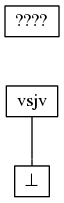
\includegraphics[scale=0.5]{resources/graphs/iteration_4.png}
\end{figure}
Het volgende voorbeeld $4$ is een tweede voorbeeld dat positief beoordeeld is. We generaliseren $[v,s,j,v]$ tot een hypothese die ook het nieuwe voorbeeld omvat. Hiervoor zijn twee mogelijkheden die we beide toevoegen zoals beschreven in figuur \ref{iter_4}.
\begin{itemize}
\item $G = \{[?,v,?,j],[v,?,?,r],[?,z,j,?],[?,z,?,v]\}$
\item $S = \{[v,?,s,r],[v,?,s,a]\}$
\end{itemize}
\subsection{Iteratie 5}
\begin{figure}
[H]
\centering
\caption{Iteratie 5}
\label{iter_5}
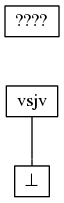
\includegraphics[scale=0.5]{resources/graphs/iteration_5.png}
\end{figure}
In iteratie 5 behandelen we ten slotte nog een positief voorbeeld. Deze keer wordt er maar \'e\'en hypothese toegevoegd en deze wordt meteen al weer verwijderd omdat ze een generalisatie is van $[v,?,s,r]$ en dus redundant is. De beschrijving van deze iteratie is te vinden in figuur \ref{iter_5}. Het resultaat van het version spaces algoritme zien we in figuur \ref{resultaat}.
\begin{itemize}
\item $G = \{[?,v,?,j],[v,?,?,r],[?,z,j,?],[?,z,?,v]\}$
\item $S = \{[v,?,s,r],[v,?,s,a]\}$
\item Gesnoeid: $[v,?,s,?]$
\end{itemize}
\begin{figure}
[H]
\centering
\caption{Resultaat}
\label{resultaat}
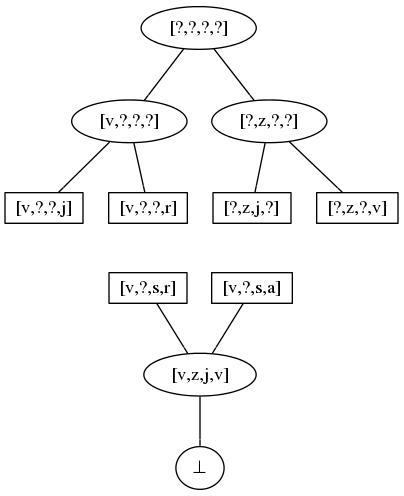
\includegraphics[scale=0.5]{resources/graphs/resultaat.png}
\end{figure}


\subsection{beslissingsprocedure}
De dame die aan het eind van de dag binnenkomt wordt als $[v,j,j,j]$ gecategoriseerd.
We kijken nu naar $S\cup G$ en zien dat deze persoon aan \'e\'en hypothesen voldoet en niet aan de vijf andere. Als we ervan uitgaan dat elke hypothese evenveel waard is kunnen we besluiten dat de cli\"ent deze dame met een grotere kans zal afkeuren dan aanvaarden.
\end{document}